\documentclass[twoside]{book}

% Packages required by doxygen
\usepackage{calc}
\usepackage{doxygen}
\usepackage{graphicx}
\usepackage[utf8]{inputenc}
\usepackage{makeidx}
\usepackage{multicol}
\usepackage{multirow}
\usepackage{textcomp}
\usepackage[table]{xcolor}

% Font selection
\usepackage[T1]{fontenc}
\usepackage{mathptmx}
\usepackage[scaled=.90]{helvet}
\usepackage{courier}
\usepackage{amssymb}
\usepackage{sectsty}
\renewcommand{\familydefault}{\sfdefault}
\allsectionsfont{%
  \fontseries{bc}\selectfont%
  \color{darkgray}%
}
\renewcommand{\DoxyLabelFont}{%
  \fontseries{bc}\selectfont%
  \color{darkgray}%
}

% Page & text layout
\usepackage{geometry}
\geometry{%
  a4paper,%
  top=2.5cm,%
  bottom=2.5cm,%
  left=2.5cm,%
  right=2.5cm%
}
\tolerance=750
\hfuzz=15pt
\hbadness=750
\setlength{\emergencystretch}{15pt}
\setlength{\parindent}{0cm}
\setlength{\parskip}{0.2cm}
\makeatletter
\renewcommand{\paragraph}{%
  \@startsection{paragraph}{4}{0ex}{-1.0ex}{1.0ex}{%
    \normalfont\normalsize\bfseries\SS@parafont%
  }%
}
\renewcommand{\subparagraph}{%
  \@startsection{subparagraph}{5}{0ex}{-1.0ex}{1.0ex}{%
    \normalfont\normalsize\bfseries\SS@subparafont%
  }%
}
\makeatother

% Headers & footers
\usepackage{fancyhdr}
\pagestyle{fancyplain}
\fancyhead[LE]{\fancyplain{}{\bfseries\thepage}}
\fancyhead[CE]{\fancyplain{}{}}
\fancyhead[RE]{\fancyplain{}{\bfseries\leftmark}}
\fancyhead[LO]{\fancyplain{}{\bfseries\rightmark}}
\fancyhead[CO]{\fancyplain{}{}}
\fancyhead[RO]{\fancyplain{}{\bfseries\thepage}}
\fancyfoot[LE]{\fancyplain{}{}}
\fancyfoot[CE]{\fancyplain{}{}}
\fancyfoot[RE]{\fancyplain{}{\bfseries\scriptsize Generated on Thu Mar 19 2015 01\-:29\-:59 for L\-A\-B2 by Doxygen }}
\fancyfoot[LO]{\fancyplain{}{\bfseries\scriptsize Generated on Thu Mar 19 2015 01\-:29\-:59 for L\-A\-B2 by Doxygen }}
\fancyfoot[CO]{\fancyplain{}{}}
\fancyfoot[RO]{\fancyplain{}{}}
\renewcommand{\footrulewidth}{0.4pt}
\renewcommand{\chaptermark}[1]{%
  \markboth{#1}{}%
}
\renewcommand{\sectionmark}[1]{%
  \markright{\thesection\ #1}%
}

% Indices & bibliography
\usepackage{natbib}
\usepackage[titles]{tocloft}
\setcounter{tocdepth}{3}
\setcounter{secnumdepth}{5}
\makeindex

% Custom commands
\newcommand{\clearemptydoublepage}{%
  \newpage{\pagestyle{empty}\cleardoublepage}%
}


%===== C O N T E N T S =====

\begin{document}

% Titlepage & ToC
\pagenumbering{roman}
\begin{titlepage}
\vspace*{7cm}
\begin{center}%
{\Large L\-A\-B2 \\[1ex]\large 0.\-1 }\\
\vspace*{1cm}
{\large Generated by Doxygen 1.8.6}\\
\vspace*{0.5cm}
{\small Thu Mar 19 2015 01:29:59}\\
\end{center}
\end{titlepage}
\clearemptydoublepage
\tableofcontents
\clearemptydoublepage
\pagenumbering{arabic}

%--- Begin generated contents ---
\chapter{Class Index}
\section{Lista klas}
Tutaj znajdują się klasy, struktury, unie i interfejsy wraz z ich krótkimi opisami\-:\begin{DoxyCompactList}
\item\contentsline{section}{{\bf Benchmark$<$ T $>$} }{\pageref{class_benchmark}}{}
\item\contentsline{section}{{\bf Kolejka$<$ T $>$} \\*Klasa \doxyref{Kolejka}{str.}{class_kolejka} sluzy do wykonywania podstawowych operacji na Kolejce\-: dodaj,odejmij element. Przechowuje informacje o ilosci wszysktich elementow }{\pageref{class_kolejka}}{}
\item\contentsline{section}{{\bf List$<$ T $>$} \\*Klasa \doxyref{List}{str.}{class_list} sluzy do wykonywania podstawowych operacji na Liscie\-: dodaj,odejmij element. Przechowuje informacje o ilosci wszysktich elementow }{\pageref{class_list}}{}
\item\contentsline{section}{{\bf Node$<$ T $>$} }{\pageref{struct_node}}{}
\item\contentsline{section}{{\bf Node\-L$<$ T $>$} }{\pageref{struct_node_l}}{}
\item\contentsline{section}{{\bf Node\-T$<$ Klucz, T $>$} }{\pageref{class_node_t}}{}
\item\contentsline{section}{{\bf Stack$<$ T $>$} }{\pageref{class_stack}}{}
\item\contentsline{section}{{\bf Tablica\-Asocjacyjna} }{\pageref{class_tablica_asocjacyjna}}{}
\end{DoxyCompactList}

\chapter{File Index}
\section{Lista plików}
Tutaj znajduje się lista wszystkich plików z ich krótkimi opisami\-:\begin{DoxyCompactList}
\item\contentsline{section}{{\bf Benchmark.\-hh} \\*Klasa \doxyref{Benchmark}{str.}{class_benchmark} sluzy do przechowywania wynikow zlozonosci obliczeniowej i danych wejsciowych,generowania liczb rozkladu Gaussowego }{\pageref{_benchmark_8hh}}{}
\item\contentsline{section}{{\bf Kolejka.\-hh} \\*Struktura przechowujaca wartosc wezla i wskaznik na nastepny element typu \doxyref{Node}{str.}{struct_node} }{\pageref{_kolejka_8hh}}{}
\item\contentsline{section}{{\bf Lista.\-hh} \\*Struktura przechowujaca wartosc wezla i wskaznik na nastepny element typu \doxyref{Node}{str.}{struct_node} }{\pageref{_lista_8hh}}{}
\item\contentsline{section}{{\bf main.\-cpp} }{\pageref{main_8cpp}}{}
\item\contentsline{section}{{\bf main3.\-cpp} }{\pageref{main3_8cpp}}{}
\item\contentsline{section}{{\bf Operacje\-Na\-Plikach.\-hh} }{\pageref{_operacje_na_plikach_8hh}}{}
\item\contentsline{section}{{\bf Sortowanie.\-cpp} }{\pageref{_sortowanie_8cpp}}{}
\item\contentsline{section}{{\bf Sortowanie.\-hh} }{\pageref{_sortowanie_8hh}}{}
\item\contentsline{section}{{\bf Stack.\-hh} \\*Klasa \doxyref{Stack}{str.}{class_stack} sluzy do przechowywania, dodawania,zdejmowania kolejnych elementow stosu }{\pageref{_stack_8hh}}{}
\item\contentsline{section}{{\bf Struktury.\-hh} }{\pageref{_struktury_8hh}}{}
\item\contentsline{section}{{\bf Zapisz\-Stos\-Kolejka\-Lista.\-cpp} }{\pageref{_zapisz_stos_kolejka_lista_8cpp}}{}
\item\contentsline{section}{{\bf Zapisz\-Stos\-Kolejka\-Lista.\-hh} }{\pageref{_zapisz_stos_kolejka_lista_8hh}}{}
\end{DoxyCompactList}

\chapter{Class Documentation}
\section{Kolejka$<$ T $>$ Class Template Reference}
\label{class_kolejka}\index{Kolejka$<$ T $>$@{Kolejka$<$ T $>$}}


klasa \doxyref{Kolejka}{p.}{class_kolejka} sluzy do wykonywania podstawowych operacji na Kolejce\-: dodaj,odejmij element. Przechowuje informacje o ilosci wszysktich elementow.  




{\ttfamily \#include $<$Kolejka.\-hh$>$}

\subsection*{Public Member Functions}
\begin{DoxyCompactItemize}
\item 
{\bf Kolejka} ()
\item 
{\bf $\sim$\-Kolejka} ()
\item 
int {\bf size} ()
\item 
void {\bf push\-\_\-front} (T value)
\item 
void {\bf pop\-\_\-back} ()
\item 
void {\bf show} ()
\end{DoxyCompactItemize}


\subsection{Detailed Description}
\subsubsection*{template$<$typename T$>$class Kolejka$<$ T $>$}

klasa \doxyref{Kolejka}{p.}{class_kolejka} sluzy do wykonywania podstawowych operacji na Kolejce\-: dodaj,odejmij element. Przechowuje informacje o ilosci wszysktich elementow. 

Definition at line 21 of file Kolejka.\-hh.



\subsection{Constructor \& Destructor Documentation}
\index{Kolejka@{Kolejka}!Kolejka@{Kolejka}}
\index{Kolejka@{Kolejka}!Kolejka@{Kolejka}}
\subsubsection[{Kolejka}]{\setlength{\rightskip}{0pt plus 5cm}template$<$typename T $>$ {\bf Kolejka}$<$ T $>$\-::{\bf Kolejka} (
\begin{DoxyParamCaption}
{}
\end{DoxyParamCaption}
)}\label{class_kolejka_a576eb7abc018d1adc1040285fda27c43}
brief Konstruktor bezparametryczny

Konstruktor bezparametryczny, ustawia parametry na 0 

Definition at line 59 of file Kolejka.\-hh.

\index{Kolejka@{Kolejka}!$\sim$\-Kolejka@{$\sim$\-Kolejka}}
\index{$\sim$\-Kolejka@{$\sim$\-Kolejka}!Kolejka@{Kolejka}}
\subsubsection[{$\sim$\-Kolejka}]{\setlength{\rightskip}{0pt plus 5cm}template$<$typename T $>$ {\bf Kolejka}$<$ T $>$\-::$\sim${\bf Kolejka} (
\begin{DoxyParamCaption}
{}
\end{DoxyParamCaption}
)}\label{class_kolejka_a5d3334a50106d57d2465522fb58701c0}
Destruktor, usuwa kolejne elementy kolejki zaczynajac od poczatku 

Definition at line 69 of file Kolejka.\-hh.



\subsection{Member Function Documentation}
\index{Kolejka@{Kolejka}!pop\-\_\-back@{pop\-\_\-back}}
\index{pop\-\_\-back@{pop\-\_\-back}!Kolejka@{Kolejka}}
\subsubsection[{pop\-\_\-back}]{\setlength{\rightskip}{0pt plus 5cm}template$<$typename T $>$ void {\bf Kolejka}$<$ T $>$\-::pop\-\_\-back (
\begin{DoxyParamCaption}
{}
\end{DoxyParamCaption}
)}\label{class_kolejka_a1c5bf50cc1431b0e6af20ee3289699e6}
brief Funkcja zdejmuje element z konca kolejki

Funkcja usuwa element z konca kolejki \begin{DoxyPrecond}{Precondition}
\doxyref{Kolejka}{p.}{class_kolejka} nie moze byc pusta 
\end{DoxyPrecond}


Definition at line 106 of file Kolejka.\-hh.

\index{Kolejka@{Kolejka}!push\-\_\-front@{push\-\_\-front}}
\index{push\-\_\-front@{push\-\_\-front}!Kolejka@{Kolejka}}
\subsubsection[{push\-\_\-front}]{\setlength{\rightskip}{0pt plus 5cm}template$<$typename T $>$ void {\bf Kolejka}$<$ T $>$\-::push\-\_\-front (
\begin{DoxyParamCaption}
\item[{T}]{value}
\end{DoxyParamCaption}
)}\label{class_kolejka_a9fe17cfd429e3a29373a1e0d229733ea}
brief Funkcja dodaje element na poczatek kolejki

Funkcja sluzy do dodania elementu na poczatek kolejki 
\begin{DoxyParams}[1]{Parameters}
\mbox{\tt in}  & {\em value-\/typ} & int, wartosc elementu zmiennej dodanej do kolejki \\
\hline
\end{DoxyParams}


Definition at line 92 of file Kolejka.\-hh.

\index{Kolejka@{Kolejka}!show@{show}}
\index{show@{show}!Kolejka@{Kolejka}}
\subsubsection[{show}]{\setlength{\rightskip}{0pt plus 5cm}template$<$typename T $>$ void {\bf Kolejka}$<$ T $>$\-::show (
\begin{DoxyParamCaption}
{}
\end{DoxyParamCaption}
)}\label{class_kolejka_a929496e3ada70f837b1672fe2170c0a4}
brief Funkcja wyswietla wszystkie elementy na standardowe wyjscie

Funkcja wyswietla elementy kolejki 

Definition at line 134 of file Kolejka.\-hh.

\index{Kolejka@{Kolejka}!size@{size}}
\index{size@{size}!Kolejka@{Kolejka}}
\subsubsection[{size}]{\setlength{\rightskip}{0pt plus 5cm}template$<$typename T $>$ int {\bf Kolejka}$<$ T $>$\-::size (
\begin{DoxyParamCaption}
{}
\end{DoxyParamCaption}
)}\label{class_kolejka_a9992a77318d031852cda3d28fd1f80b3}
brief Funkcja zwraca rozmiar kolejki

\begin{DoxyReturn}{Returns}
Funkcja zwraca wartosc rozmiaru kolejki 
\end{DoxyReturn}


Definition at line 82 of file Kolejka.\-hh.



The documentation for this class was generated from the following file\-:\begin{DoxyCompactItemize}
\item 
inc/{\bf Kolejka.\-hh}\end{DoxyCompactItemize}

\section{Dokumentacja szablonu klasy List$<$ T $>$}
\label{class_list}\index{List$<$ T $>$@{List$<$ T $>$}}


klasa \doxyref{List}{str.}{class_list} sluzy do wykonywania podstawowych operacji na Liscie\-: dodaj,odejmij element. Przechowuje informacje o ilosci wszysktich elementow.  




{\ttfamily \#include $<$Lista.\-hh$>$}



Diagram dziedziczenia dla List$<$ T $>$
\nopagebreak
\begin{figure}[H]
\begin{center}
\leavevmode
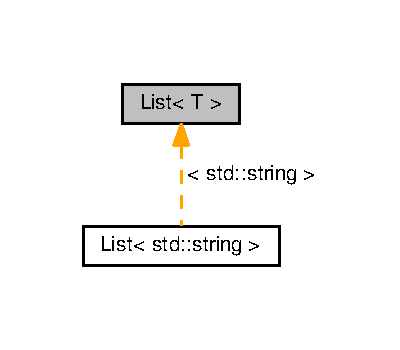
\includegraphics[width=192pt]{class_list__inherit__graph}
\end{center}
\end{figure}
\subsection*{Metody publiczne}
\begin{DoxyCompactItemize}
\item 
{\bf List} ()
\item 
{\bf $\sim$\-List} ()
\item 
int {\bf size} ()
\item 
void {\bf push\-\_\-front} (T value)
\item 
void {\bf pop\-\_\-front} ()
\item 
void {\bf push\-\_\-back} (T value)
\item 
void {\bf pop\-\_\-back} ()
\item 
void {\bf show} ()
\item 
void {\bf show\-Od\-Konca} ()
\item 
void {\bf push} (T value, int nr=0)
\item 
T \& {\bf operator[$\,$]} (int a)
\end{DoxyCompactItemize}
\subsection*{Atrybuty publiczne}
\begin{DoxyCompactItemize}
\item 
{\bf Node\-L}$<$ T $>$ $\ast$ {\bf head}
\item 
{\bf Node\-L}$<$ T $>$ $\ast$ {\bf tail}
\item 
int {\bf \-\_\-size}
\end{DoxyCompactItemize}


\subsection{Opis szczegółowy}
\subsubsection*{template$<$typename T$>$class List$<$ T $>$}



Definicja w linii 25 pliku Lista.\-hh.



\subsection{Dokumentacja konstruktora i destruktora}
\index{List@{List}!List@{List}}
\index{List@{List}!List@{List}}
\subsubsection[{List}]{\setlength{\rightskip}{0pt plus 5cm}template$<$typename T $>$ {\bf List}$<$ T $>$\-::{\bf List} (
\begin{DoxyParamCaption}
{}
\end{DoxyParamCaption}
)}\label{class_list_a5c5e27671b21b3815d4e25b953c69454}
brief Konstruktor bezparametryczny

Konstruktor bezparametryczny, ustawia parametry na 0 

Definicja w linii 101 pliku Lista.\-hh.

\index{List@{List}!$\sim$\-List@{$\sim$\-List}}
\index{$\sim$\-List@{$\sim$\-List}!List@{List}}
\subsubsection[{$\sim$\-List}]{\setlength{\rightskip}{0pt plus 5cm}template$<$typename T $>$ {\bf List}$<$ T $>$\-::$\sim${\bf List} (
\begin{DoxyParamCaption}
{}
\end{DoxyParamCaption}
)}\label{class_list_a2b58189090f6e5ce52939c9195e59e85}
brief Destruktor

Destruktor, usuwa kolejne elementy listy zaczynajac od poczatku 

Definicja w linii 112 pliku Lista.\-hh.



\subsection{Dokumentacja funkcji składowych}
\index{List@{List}!operator[$\,$]@{operator[]}}
\index{operator[$\,$]@{operator[]}!List@{List}}
\subsubsection[{operator[]}]{\setlength{\rightskip}{0pt plus 5cm}template$<$typename T$>$ T\& {\bf List}$<$ T $>$\-::operator[$\,$] (
\begin{DoxyParamCaption}
\item[{int}]{a}
\end{DoxyParamCaption}
)\hspace{0.3cm}{\ttfamily [inline]}}\label{class_list_a52f00da87e26da27b3569389ec692e83}
Przeciazony operator indeksowania zwraca referencje do elementu o indeksie a 

Definicja w linii 87 pliku Lista.\-hh.

\index{List@{List}!pop\-\_\-back@{pop\-\_\-back}}
\index{pop\-\_\-back@{pop\-\_\-back}!List@{List}}
\subsubsection[{pop\-\_\-back}]{\setlength{\rightskip}{0pt plus 5cm}template$<$typename T $>$ void {\bf List}$<$ T $>$\-::pop\-\_\-back (
\begin{DoxyParamCaption}
{}
\end{DoxyParamCaption}
)}\label{class_list_a42e1aee3e26b76b3f4d9386efa7fe8b7}
brief Funkcja zdejmuje element z konca listy

Funkcja usuwa element z konca listy \begin{DoxyPrecond}{Warunek wstępny}
Lista nie moze byc pusta 
\end{DoxyPrecond}


Definicja w linii 229 pliku Lista.\-hh.

\index{List@{List}!pop\-\_\-front@{pop\-\_\-front}}
\index{pop\-\_\-front@{pop\-\_\-front}!List@{List}}
\subsubsection[{pop\-\_\-front}]{\setlength{\rightskip}{0pt plus 5cm}template$<$typename T $>$ void {\bf List}$<$ T $>$\-::pop\-\_\-front (
\begin{DoxyParamCaption}
{}
\end{DoxyParamCaption}
)}\label{class_list_a024af4543f71544345351a45850c42d8}
brief Funkcja zdejmuje element z poczatku listy

Funkcja usuwa element z poczatku listy \begin{DoxyPrecond}{Warunek wstępny}
Lista nie moze byc pusta 
\end{DoxyPrecond}


Definicja w linii 152 pliku Lista.\-hh.

\index{List@{List}!push@{push}}
\index{push@{push}!List@{List}}
\subsubsection[{push}]{\setlength{\rightskip}{0pt plus 5cm}template$<$typename T$>$ void {\bf List}$<$ T $>$\-::push (
\begin{DoxyParamCaption}
\item[{T}]{value, }
\item[{int}]{nr = {\ttfamily 0}}
\end{DoxyParamCaption}
)}\label{class_list_a3bf27eb40044a3586f25899aa428c0c6}
brief Funkcja dodaje element przed elementem o indeksie nr

Funkcja dodaje element przed elementem o indeksie nr 
\begin{DoxyParams}[1]{Parametry}
\mbox{\tt in}  & {\em value-\/wybrany} & typ, wartosc elementu dodanego do listy \\
\hline
\mbox{\tt in}  & {\em nr-\/} & indeks elementu przed ktorym ma byc dodany element \\
\hline
\end{DoxyParams}
\begin{DoxyPrecond}{Warunek wstępny}
indeksowanie od 0 
\end{DoxyPrecond}


Definicja w linii 196 pliku Lista.\-hh.

\index{List@{List}!push\-\_\-back@{push\-\_\-back}}
\index{push\-\_\-back@{push\-\_\-back}!List@{List}}
\subsubsection[{push\-\_\-back}]{\setlength{\rightskip}{0pt plus 5cm}template$<$typename T$>$ void {\bf List}$<$ T $>$\-::push\-\_\-back (
\begin{DoxyParamCaption}
\item[{T}]{value}
\end{DoxyParamCaption}
)}\label{class_list_a6c3e359bceddd875f6d27e75de7ed15d}
brief Funkcja dodaje element na koniec listy

Funkcja dodaje element na koniec listy 
\begin{DoxyParams}[1]{Parametry}
\mbox{\tt in}  & {\em value} & -\/ typ int, wartosc elementu dodanego na koniec listy \\
\hline
\end{DoxyParams}


Definicja w linii 171 pliku Lista.\-hh.



Oto graf wywoływań tej funkcji\-:
\nopagebreak
\begin{figure}[H]
\begin{center}
\leavevmode
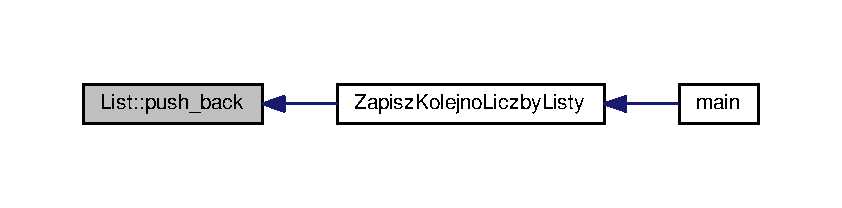
\includegraphics[width=330pt]{class_list_a6c3e359bceddd875f6d27e75de7ed15d_icgraph}
\end{center}
\end{figure}


\index{List@{List}!push\-\_\-front@{push\-\_\-front}}
\index{push\-\_\-front@{push\-\_\-front}!List@{List}}
\subsubsection[{push\-\_\-front}]{\setlength{\rightskip}{0pt plus 5cm}template$<$typename T$>$ void {\bf List}$<$ T $>$\-::push\-\_\-front (
\begin{DoxyParamCaption}
\item[{T}]{value}
\end{DoxyParamCaption}
)}\label{class_list_a2b4c57456c11a4d95bf039ae2d4e1e3c}
brief Funkcja dodaje element na poczatek listy

Funkcja sluzy do dodania elementu na poczatek listy 
\begin{DoxyParams}[1]{Parametry}
\mbox{\tt in}  & {\em value-\/typ} & int, wartosc elementu zmiennej dodanej do listy \\
\hline
\end{DoxyParams}


Definicja w linii 135 pliku Lista.\-hh.



Oto graf wywoływań tej funkcji\-:
\nopagebreak
\begin{figure}[H]
\begin{center}
\leavevmode
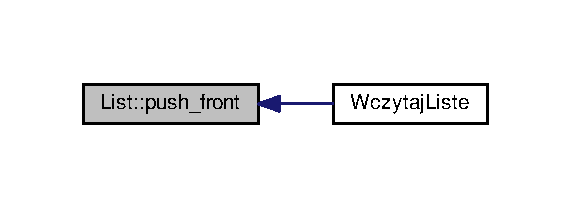
\includegraphics[width=274pt]{class_list_a2b4c57456c11a4d95bf039ae2d4e1e3c_icgraph}
\end{center}
\end{figure}


\index{List@{List}!show@{show}}
\index{show@{show}!List@{List}}
\subsubsection[{show}]{\setlength{\rightskip}{0pt plus 5cm}template$<$typename T $>$ void {\bf List}$<$ T $>$\-::show (
\begin{DoxyParamCaption}
{}
\end{DoxyParamCaption}
)}\label{class_list_aeed4e21c08aa25bf4fe12a2ac96c0f1f}
brief Funkcja wyswietla wszystkie elementy na standardowe wyjscie

brief Funkcja pokazujaca na strumieniu std\-::cout zawartosc listy

Funkcja wyswietla elementy listy 

Definicja w linii 259 pliku Lista.\-hh.

\index{List@{List}!show\-Od\-Konca@{show\-Od\-Konca}}
\index{show\-Od\-Konca@{show\-Od\-Konca}!List@{List}}
\subsubsection[{show\-Od\-Konca}]{\setlength{\rightskip}{0pt plus 5cm}template$<$typename T $>$ void {\bf List}$<$ T $>$\-::show\-Od\-Konca (
\begin{DoxyParamCaption}
{}
\end{DoxyParamCaption}
)}\label{class_list_aeecf3b2e13b4e2489c4974aacd318b33}
brief Funkcja pokazujaca na strumieniu std\-::cout zawartosc listy od konca

Funkcja wyswietla elementy listy od konca 

Definicja w linii 273 pliku Lista.\-hh.

\index{List@{List}!size@{size}}
\index{size@{size}!List@{List}}
\subsubsection[{size}]{\setlength{\rightskip}{0pt plus 5cm}template$<$typename T $>$ int {\bf List}$<$ T $>$\-::size (
\begin{DoxyParamCaption}
{}
\end{DoxyParamCaption}
)}\label{class_list_a2497bdf42246d61237aaf046c116183a}
brief Funkcja zwraca rozmiar listy

\begin{DoxyReturn}{Zwraca}
Funkcja zwraca wartosc rozmiaru listy 
\end{DoxyReturn}


Definicja w linii 125 pliku Lista.\-hh.



\subsection{Dokumentacja atrybutów składowych}
\index{List@{List}!\-\_\-size@{\-\_\-size}}
\index{\-\_\-size@{\-\_\-size}!List@{List}}
\subsubsection[{\-\_\-size}]{\setlength{\rightskip}{0pt plus 5cm}template$<$typename T$>$ int {\bf List}$<$ T $>$\-::\-\_\-size}\label{class_list_ad56fcbd2da2271dce020bb933349cba4}
brief Informacja o rozmiarze listy 

Definicja w linii 39 pliku Lista.\-hh.

\index{List@{List}!head@{head}}
\index{head@{head}!List@{List}}
\subsubsection[{head}]{\setlength{\rightskip}{0pt plus 5cm}template$<$typename T$>$ {\bf Node\-L}$<$T$>$$\ast$ {\bf List}$<$ T $>$\-::head}\label{class_list_a3caa8173609b10b902f3a578975211d6}
brief wskaznik do ktorego doczepione sa kolejne elementy listy 

Definicja w linii 31 pliku Lista.\-hh.

\index{List@{List}!tail@{tail}}
\index{tail@{tail}!List@{List}}
\subsubsection[{tail}]{\setlength{\rightskip}{0pt plus 5cm}template$<$typename T$>$ {\bf Node\-L}$<$T$>$$\ast$ {\bf List}$<$ T $>$\-::tail}\label{class_list_a40495d6470191f412dc9b51efeae43c5}
brief wskaznik pokazujacy na koniec listy 

Definicja w linii 35 pliku Lista.\-hh.



Dokumentacja dla tej klasy została wygenerowana z pliku\-:\begin{DoxyCompactItemize}
\item 
{\bf Lista.\-hh}\end{DoxyCompactItemize}

\section{Dokumentacja szablonu struktury Node$<$ T $>$}
\label{struct_node}\index{Node$<$ T $>$@{Node$<$ T $>$}}


{\ttfamily \#include $<$Kolejka.\-hh$>$}

\subsection*{Atrybuty publiczne}
\begin{DoxyCompactItemize}
\item 
T {\bf val}
\item 
{\bf Node}$<$ T $>$ $\ast$ {\bf next}
\end{DoxyCompactItemize}


\subsection{Opis szczegółowy}
\subsubsection*{template$<$typename T$>$struct Node$<$ T $>$}



Definicja w linii 10 pliku Kolejka.\-hh.



\subsection{Dokumentacja atrybutów składowych}
\index{Node@{Node}!next@{next}}
\index{next@{next}!Node@{Node}}
\subsubsection[{next}]{\setlength{\rightskip}{0pt plus 5cm}template$<$typename T$>$ {\bf Node}$<$T$>$$\ast$ {\bf Node}$<$ T $>$\-::next}\label{struct_node_a8bedac90cd0aedd2847dd49f671d4d4a}


Definicja w linii 13 pliku Kolejka.\-hh.

\index{Node@{Node}!val@{val}}
\index{val@{val}!Node@{Node}}
\subsubsection[{val}]{\setlength{\rightskip}{0pt plus 5cm}template$<$typename T$>$ T {\bf Node}$<$ T $>$\-::val}\label{struct_node_a63ca7703bf78a4ea3f6a7f32a9f705c8}


Definicja w linii 12 pliku Kolejka.\-hh.



Dokumentacja dla tej struktury została wygenerowana z pliku\-:\begin{DoxyCompactItemize}
\item 
{\bf Kolejka.\-hh}\end{DoxyCompactItemize}

\section{Node\-L$<$ T $>$ Struct Template Reference}
\label{struct_node_l}\index{Node\-L$<$ T $>$@{Node\-L$<$ T $>$}}


{\ttfamily \#include $<$Lista.\-hh$>$}

\subsection*{Public Attributes}
\begin{DoxyCompactItemize}
\item 
T {\bf val}
\item 
{\bf Node\-L}$<$ T $>$ $\ast$ {\bf next}
\end{DoxyCompactItemize}


\subsection{Detailed Description}
\subsubsection*{template$<$typename T$>$struct Node\-L$<$ T $>$}



Definition at line 11 of file Lista.\-hh.



\subsection{Member Data Documentation}
\index{Node\-L@{Node\-L}!next@{next}}
\index{next@{next}!NodeL@{Node\-L}}
\subsubsection[{next}]{\setlength{\rightskip}{0pt plus 5cm}template$<$typename T$>$ {\bf Node\-L}$<$T$>$$\ast$ {\bf Node\-L}$<$ T $>$\-::next}\label{struct_node_l_a0c3afc9e532c18b261ead8ee2218100d}


Definition at line 14 of file Lista.\-hh.

\index{Node\-L@{Node\-L}!val@{val}}
\index{val@{val}!NodeL@{Node\-L}}
\subsubsection[{val}]{\setlength{\rightskip}{0pt plus 5cm}template$<$typename T$>$ T {\bf Node\-L}$<$ T $>$\-::val}\label{struct_node_l_af8d6352b8a3b463d1a1f2dc9fa6378d6}


Definition at line 13 of file Lista.\-hh.



The documentation for this struct was generated from the following file\-:\begin{DoxyCompactItemize}
\item 
inc/{\bf Lista.\-hh}\end{DoxyCompactItemize}

\section{Dokumentacja szablonu klasy Stack$<$ T $>$}
\label{class_stack}\index{Stack$<$ T $>$@{Stack$<$ T $>$}}


{\ttfamily \#include $<$Stack.\-hh$>$}

\subsection*{Metody publiczne}
\begin{DoxyCompactItemize}
\item 
{\bf Stack} (int {\bf capacity}=10)
\item 
void {\bf push} (T value)
\item 
T {\bf peek} ()
\item 
int {\bf size} ()
\item 
{\bf $\sim$\-Stack} ()
\item 
void {\bf pop} ()
\item 
T \& {\bf operator[$\,$]} (int a)
\end{DoxyCompactItemize}
\subsection*{Atrybuty publiczne}
\begin{DoxyCompactItemize}
\item 
T $\ast$ {\bf top}
\item 
int {\bf capacity}
\item 
T $\ast$ {\bf storage}
\end{DoxyCompactItemize}


\subsection{Opis szczegółowy}
\subsubsection*{template$<$typename T$>$class Stack$<$ T $>$}



Definicja w linii 11 pliku Stack.\-hh.



\subsection{Dokumentacja konstruktora i destruktora}
\index{Stack@{Stack}!Stack@{Stack}}
\index{Stack@{Stack}!Stack@{Stack}}
\subsubsection[{Stack}]{\setlength{\rightskip}{0pt plus 5cm}template$<$typename T $>$ {\bf Stack}$<$ T $>$\-::{\bf Stack} (
\begin{DoxyParamCaption}
\item[{int}]{capacity = {\ttfamily 10}}
\end{DoxyParamCaption}
)}\label{class_stack_ae6f58b476da16d508f90841455a09e5a}
Konstruktor parametryczny klasy \doxyref{Stack}{str.}{class_stack} 
\begin{DoxyParams}[1]{Parametry}
\mbox{\tt in}  & {\em capacity} & -\/ typ int, rozmiar stosu \\
\hline
\end{DoxyParams}


Definicja w linii 66 pliku Stack.\-hh.

\index{Stack@{Stack}!$\sim$\-Stack@{$\sim$\-Stack}}
\index{$\sim$\-Stack@{$\sim$\-Stack}!Stack@{Stack}}
\subsubsection[{$\sim$\-Stack}]{\setlength{\rightskip}{0pt plus 5cm}template$<$typename T $>$ {\bf Stack}$<$ T $>$\-::$\sim${\bf Stack} (
\begin{DoxyParamCaption}
{}
\end{DoxyParamCaption}
)}\label{class_stack_a9e7a00875aefbdac560ab189b7bc61d1}
Destruktor klasy \doxyref{Stack}{str.}{class_stack} 

Definicja w linii 125 pliku Stack.\-hh.



\subsection{Dokumentacja funkcji składowych}
\index{Stack@{Stack}!operator[$\,$]@{operator[]}}
\index{operator[$\,$]@{operator[]}!Stack@{Stack}}
\subsubsection[{operator[]}]{\setlength{\rightskip}{0pt plus 5cm}template$<$typename T$>$ T\& {\bf Stack}$<$ T $>$\-::operator[$\,$] (
\begin{DoxyParamCaption}
\item[{int}]{a}
\end{DoxyParamCaption}
)\hspace{0.3cm}{\ttfamily [inline]}}\label{class_stack_aa1bb812d47701510f830fa3ff36c47ad}
brief Przeciazony operator indeksowania, umozliwia traktowanie stosu jak tablicy 

Definicja w linii 54 pliku Stack.\-hh.

\index{Stack@{Stack}!peek@{peek}}
\index{peek@{peek}!Stack@{Stack}}
\subsubsection[{peek}]{\setlength{\rightskip}{0pt plus 5cm}template$<$typename T $>$ T {\bf Stack}$<$ T $>$\-::peek (
\begin{DoxyParamCaption}
{}
\end{DoxyParamCaption}
)}\label{class_stack_adcb4774ac8aa94cbc19b461da9bdee3a}
Funkcja pokazuje element znajdujacy sie na szczycie stosu \begin{DoxyPrecond}{Warunek wstępny}
Stos nie moze byc pusty 
\end{DoxyPrecond}


Definicja w linii 104 pliku Stack.\-hh.

\index{Stack@{Stack}!pop@{pop}}
\index{pop@{pop}!Stack@{Stack}}
\subsubsection[{pop}]{\setlength{\rightskip}{0pt plus 5cm}template$<$typename T $>$ void {\bf Stack}$<$ T $>$\-::pop (
\begin{DoxyParamCaption}
{}
\end{DoxyParamCaption}
)}\label{class_stack_a2723aec5c7e2611b97fcffeb7709de33}
Funkcja pop zdejmuje ostatni element ze stosu \begin{DoxyPrecond}{Warunek wstępny}
Stos nie moze byc pusty 
\end{DoxyPrecond}


Definicja w linii 136 pliku Stack.\-hh.

\index{Stack@{Stack}!push@{push}}
\index{push@{push}!Stack@{Stack}}
\subsubsection[{push}]{\setlength{\rightskip}{0pt plus 5cm}template$<$typename T $>$ void {\bf Stack}$<$ T $>$\-::push (
\begin{DoxyParamCaption}
\item[{T}]{value}
\end{DoxyParamCaption}
)}\label{class_stack_a892e33693ec391dd20c09a978b038a87}
Funkcja dodaje element na koniec tablicy stosu 
\begin{DoxyParams}[1]{Parametry}
\mbox{\tt in}  & {\em value} & -\/ typ int, wartosc dodana do stosu \\
\hline
\end{DoxyParams}
\begin{DoxyPostcond}{Warunek końcowy}
wykorzystana metoda podwajania do powiekszania stosu 
\end{DoxyPostcond}


Definicja w linii 83 pliku Stack.\-hh.



Oto graf wywoływań tej funkcji\-:
\nopagebreak
\begin{figure}[H]
\begin{center}
\leavevmode
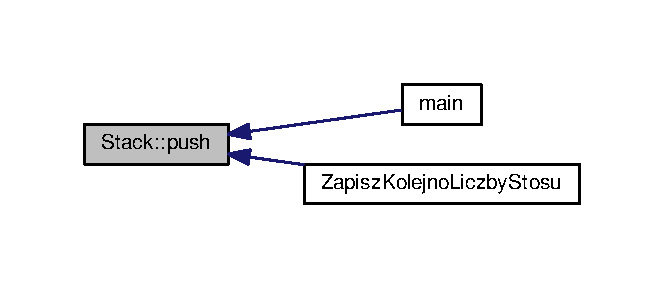
\includegraphics[width=318pt]{class_stack_a892e33693ec391dd20c09a978b038a87_icgraph}
\end{center}
\end{figure}


\index{Stack@{Stack}!size@{size}}
\index{size@{size}!Stack@{Stack}}
\subsubsection[{size}]{\setlength{\rightskip}{0pt plus 5cm}template$<$typename T $>$ int {\bf Stack}$<$ T $>$\-::size (
\begin{DoxyParamCaption}
{}
\end{DoxyParamCaption}
)}\label{class_stack_a3091d98f798b1b3e69b644d5b778c428}
Funkcja pokazuje ilosc elementow stosu \begin{DoxyReturn}{Zwraca}
zwraca ilosc elementow stosu 
\end{DoxyReturn}


Definicja w linii 116 pliku Stack.\-hh.



\subsection{Dokumentacja atrybutów składowych}
\index{Stack@{Stack}!capacity@{capacity}}
\index{capacity@{capacity}!Stack@{Stack}}
\subsubsection[{capacity}]{\setlength{\rightskip}{0pt plus 5cm}template$<$typename T$>$ int {\bf Stack}$<$ T $>$\-::capacity}\label{class_stack_a137ebd3966a796919ae064d3b205126c}


Definicja w linii 21 pliku Stack.\-hh.

\index{Stack@{Stack}!storage@{storage}}
\index{storage@{storage}!Stack@{Stack}}
\subsubsection[{storage}]{\setlength{\rightskip}{0pt plus 5cm}template$<$typename T$>$ T$\ast$ {\bf Stack}$<$ T $>$\-::storage}\label{class_stack_a93b0829d076e2a2a0fe3bf1fd0995c80}


Definicja w linii 25 pliku Stack.\-hh.

\index{Stack@{Stack}!top@{top}}
\index{top@{top}!Stack@{Stack}}
\subsubsection[{top}]{\setlength{\rightskip}{0pt plus 5cm}template$<$typename T$>$ T$\ast$ {\bf Stack}$<$ T $>$\-::top}\label{class_stack_a4ff314413cff82b4343c3094423e4345}


Definicja w linii 17 pliku Stack.\-hh.



Dokumentacja dla tej klasy została wygenerowana z pliku\-:\begin{DoxyCompactItemize}
\item 
{\bf Stack.\-hh}\end{DoxyCompactItemize}

\chapter{File Documentation}
\section{Dokumentacja pliku Kolejka.\-hh}
\label{_kolejka_8hh}\index{Kolejka.\-hh@{Kolejka.\-hh}}


Struktura przechowujaca wartosc wezla i wskaznik na nastepny element typu \doxyref{Node}{str.}{struct_node}.  


Ten wykres pokazuje, które pliki bezpośrednio lub pośrednio załączają ten plik\-:\nopagebreak
\begin{figure}[H]
\begin{center}
\leavevmode
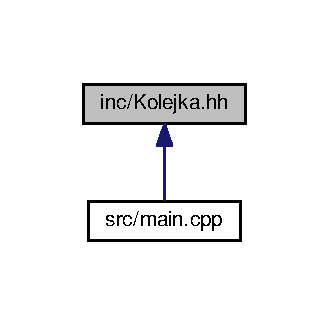
\includegraphics[width=218pt]{_kolejka_8hh__dep__incl}
\end{center}
\end{figure}
\subsection*{Komponenty}
\begin{DoxyCompactItemize}
\item 
struct {\bf Node$<$ T $>$}
\item 
class {\bf Kolejka$<$ T $>$}
\begin{DoxyCompactList}\small\item\em klasa \doxyref{Kolejka}{str.}{class_kolejka} sluzy do wykonywania podstawowych operacji na Kolejce\-: dodaj,odejmij element. Przechowuje informacje o ilosci wszysktich elementow. \end{DoxyCompactList}\end{DoxyCompactItemize}

\section{inc/\-Lista.hh File Reference}
\label{_lista_8hh}\index{inc/\-Lista.\-hh@{inc/\-Lista.\-hh}}


Struktura przechowujaca wartosc wezla i wskaznik na nastepny element typu \doxyref{Node}{p.}{struct_node}.  


This graph shows which files directly or indirectly include this file\-:\nopagebreak
\begin{figure}[H]
\begin{center}
\leavevmode
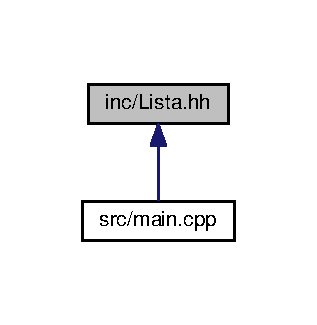
\includegraphics[width=152pt]{_lista_8hh__dep__incl}
\end{center}
\end{figure}
\subsection*{Classes}
\begin{DoxyCompactItemize}
\item 
struct {\bf Node\-L$<$ T $>$}
\item 
class {\bf List$<$ T $>$}
\begin{DoxyCompactList}\small\item\em klasa \doxyref{List}{p.}{class_list} sluzy do wykonywania podstawowych operacji na Liscie\-: dodaj,odejmij element. Przechowuje informacje o ilosci wszysktich elementow. \end{DoxyCompactList}\end{DoxyCompactItemize}


\subsection{Detailed Description}
Struktura przechowujaca wartosc wezla i wskaznik na nastepny element typu \doxyref{Node}{p.}{struct_node}. 

Definition in file {\bf Lista.\-hh}.


\section{Dokumentacja pliku Stack.\-hh}
\label{_stack_8hh}\index{Stack.\-hh@{Stack.\-hh}}


Klasa \doxyref{Stack}{str.}{class_stack} sluzy do przechowywania, dodawania,zdejmowania kolejnych elementow stosu.  


{\ttfamily \#include $<$string$>$}\\*
Wykres zależności załączania dla Stack.\-hh\-:
\nopagebreak
\begin{figure}[H]
\begin{center}
\leavevmode
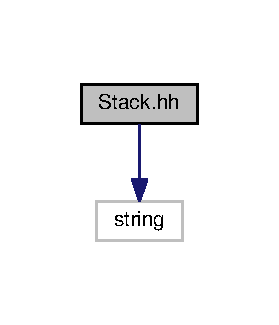
\includegraphics[width=134pt]{_stack_8hh__incl}
\end{center}
\end{figure}
Ten wykres pokazuje, które pliki bezpośrednio lub pośrednio załączają ten plik\-:
\nopagebreak
\begin{figure}[H]
\begin{center}
\leavevmode
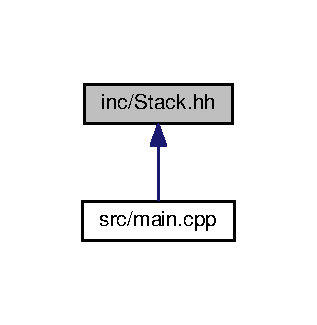
\includegraphics[width=350pt]{_stack_8hh__dep__incl}
\end{center}
\end{figure}
\subsection*{Komponenty}
\begin{DoxyCompactItemize}
\item 
class {\bf Stack$<$ T $>$}
\end{DoxyCompactItemize}
\subsection*{Funkcje}
\begin{DoxyCompactItemize}
\item 
{\footnotesize template$<$typename T $>$ }\\std\-::ostream \& {\bf operator$<$$<$} (std\-::ostream \&out, const {\bf Stack}$<$ T $>$ \&stack)
\end{DoxyCompactItemize}


\subsection{Dokumentacja funkcji}
\index{Stack.\-hh@{Stack.\-hh}!operator$<$$<$@{operator$<$$<$}}
\index{operator$<$$<$@{operator$<$$<$}!Stack.hh@{Stack.\-hh}}
\subsubsection[{operator$<$$<$}]{\setlength{\rightskip}{0pt plus 5cm}template$<$typename T $>$ std\-::ostream\& operator$<$$<$ (
\begin{DoxyParamCaption}
\item[{std\-::ostream \&}]{out, }
\item[{const {\bf Stack}$<$ T $>$ \&}]{stack}
\end{DoxyParamCaption}
)}\label{_stack_8hh_a3a3ec1f00086320ead07a87074476e81}
Funkcja operatorowa sluzy do wyswietlania stosu,zbedna 
\begin{DoxyParams}[1]{Parametry}
\mbox{\tt in}  & {\em \&out} & -\/ referencja do strumienia wyjsciowego \\
\hline
\mbox{\tt in}  & {\em \&stack-\/} & referencja do stosu \\
\hline
\end{DoxyParams}
\begin{DoxyReturn}{Zwraca}
zwraca referencje do strumienia wyjsciowego 
\end{DoxyReturn}


Definicja w linii 151 pliku Stack.\-hh.


\section{Dokumentacja pliku main.\-cpp}
\label{main_8cpp}\index{main.\-cpp@{main.\-cpp}}
{\ttfamily \#include $<$iostream$>$}\\*
{\ttfamily \#include $<$fstream$>$}\\*
{\ttfamily \#include $<$string$>$}\\*
{\ttfamily \#include $<$cstdlib$>$}\\*
{\ttfamily \#include \char`\"{}Benchmark.\-hh\char`\"{}}\\*
{\ttfamily \#include \char`\"{}Zapisz\-Stos\-Kolejka\-Lista.\-hh\char`\"{}}\\*
{\ttfamily \#include \char`\"{}Operacje\-Na\-Plikach.\-hh\char`\"{}}\\*
{\ttfamily \#include \char`\"{}Struktury.\-hh\char`\"{}}\\*
{\ttfamily \#include \char`\"{}Sortowanie.\-hh\char`\"{}}\\*
Wykres zależności załączania dla main.\-cpp\-:
\nopagebreak
\begin{figure}[H]
\begin{center}
\leavevmode
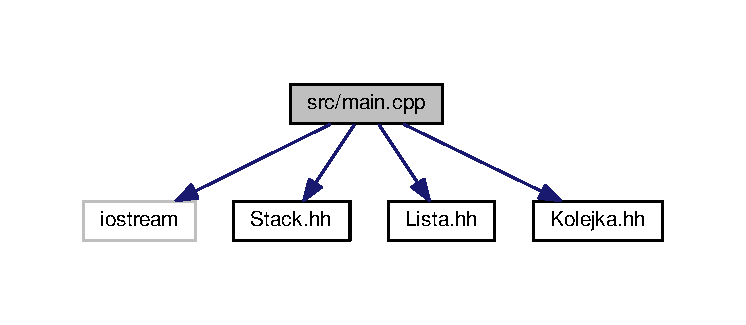
\includegraphics[width=350pt]{main_8cpp__incl}
\end{center}
\end{figure}
\subsection*{Funkcje}
\begin{DoxyCompactItemize}
\item 
int {\bf main} (int argc, char $\ast$argv[$\,$])
\end{DoxyCompactItemize}


\subsection{Dokumentacja funkcji}
\index{main.\-cpp@{main.\-cpp}!main@{main}}
\index{main@{main}!main.cpp@{main.\-cpp}}
\subsubsection[{main}]{\setlength{\rightskip}{0pt plus 5cm}int main (
\begin{DoxyParamCaption}
\item[{int}]{argc, }
\item[{char $\ast$}]{argv[$\,$]}
\end{DoxyParamCaption}
)}\label{main_8cpp_a0ddf1224851353fc92bfbff6f499fa97}


Definicja w linii 13 pliku main.\-cpp.



Oto graf wywołań dla tej funkcji\-:
\nopagebreak
\begin{figure}[H]
\begin{center}
\leavevmode
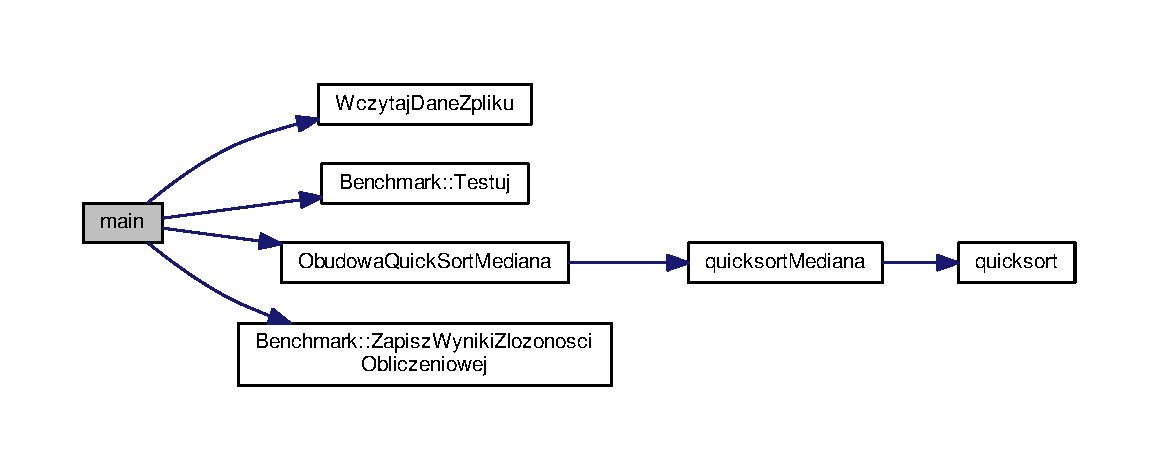
\includegraphics[width=350pt]{main_8cpp_a0ddf1224851353fc92bfbff6f499fa97_cgraph}
\end{center}
\end{figure}



%--- End generated contents ---

% Index
\newpage
\phantomsection
\addcontentsline{toc}{chapter}{Index}
\printindex

\end{document}
